\section{Low Power Wide Area Network}

Long Range Wide Area Network (LoRaWAN)  is a communication protocol tailored for low-power, long-range IoT applications.
Unlike traditional cellular networks, LoRaWAN employs an association-less communication model, allowing devices to transmit without establishing persistent links to the network infrastructure. 
The architecture comprises three primary components: end devices, gateways, and a network server.

End devices are typically deployed in the field to collect and transmit data. 
Gateways act as intermediaries, bridging the wireless transmission from end devices to the network server, which hosts most of the system intelligence. 
The network server is responsible for de-duplicating messages, managing acknowledgments, adapting radio parameters, and orchestrating overall communication to ensure reliable and energy-efficient operation.

\begin{figure}[H]
    \centering
    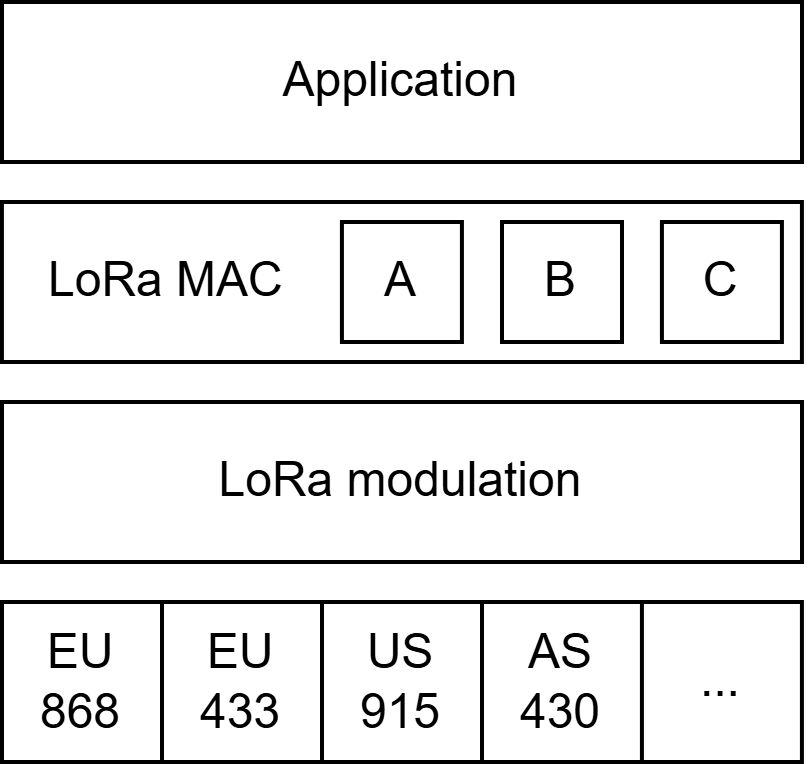
\includegraphics[width=0.4\linewidth]{images/iot11.png}
    \caption{LoraWAN protocol stack}
\end{figure}

LoRaTM employs a proprietary chirp spread spectrum modulation technique. 
This method modulates information onto chirped signals, enhancing resilience against interference and enabling long-range, low-power communication. 
The chip rate $R_C$ and bit rate $R_b$ are governed by:
\[R_C=\text{BW}\qquad R_b=\text{SF}\dfrac{4\text{BW}}{2^{\text{SF}}(4+\text{CR})}\]
Here, $\text{BW}$ is the bandwidth, $\text{SF}$ is the spreading factor, and $\text{CR}$ is the coding rate. 

There is an inherent trade-off between data rate and transmission reliability:
\begin{itemize}
    \item Lower spreading factors yield higher data rates but reduced robustness.
    \item Higher spreading factors enhance signal sensitivity and reliability, ideal for long-distance or noisy environments.
\end{itemize}
\noindent The minimum required received power for successful decoding is given by:
\[P_{\min}=-174+10\log_{10}\text{BW}+\text{NF}+\text{SNR}\]
\noindent Here, $\text{BW}$ is the reference bandwidth, $\text{NF}$ is the noise, and $\text{SNR}$ is the signal-to-noise ratio. 

\subsection{End devices}
LoRaWAN defines three operational classes for end devices, optimized for different application needs and energy constraints:
\begin{itemize}
    \item \textit{Class A}: the most energy-efficient mode. Devices initiate uplinks at will and open two short downlink reception windows afterward.
    \item \textit{Class B}: devices synchronize with periodic beacons and offer scheduled receive windows, enabling more predictable downlink communication.
    \item \textit{Class C}: devices continuously listen for downlink messages, offering the lowest latency at the cost of higher power consumption.
\end{itemize}
In the European LoRaWAN specification, the timing of Class A receive windows is fixed. 
Upon sending an uplink, the end device opens two sequential receive windows.
If a valid preamble is detected in the first window, the device remains awake until the message is demodulated. 
If the message passes address and integrity checks, the second window is skipped, minimizing power usage.

\subsection{Messages}
LoRaWAN messages are organized across several protocol layers to ensure synchronization, integrity, and proper routing.
\begin{figure}[H]
    \centering
    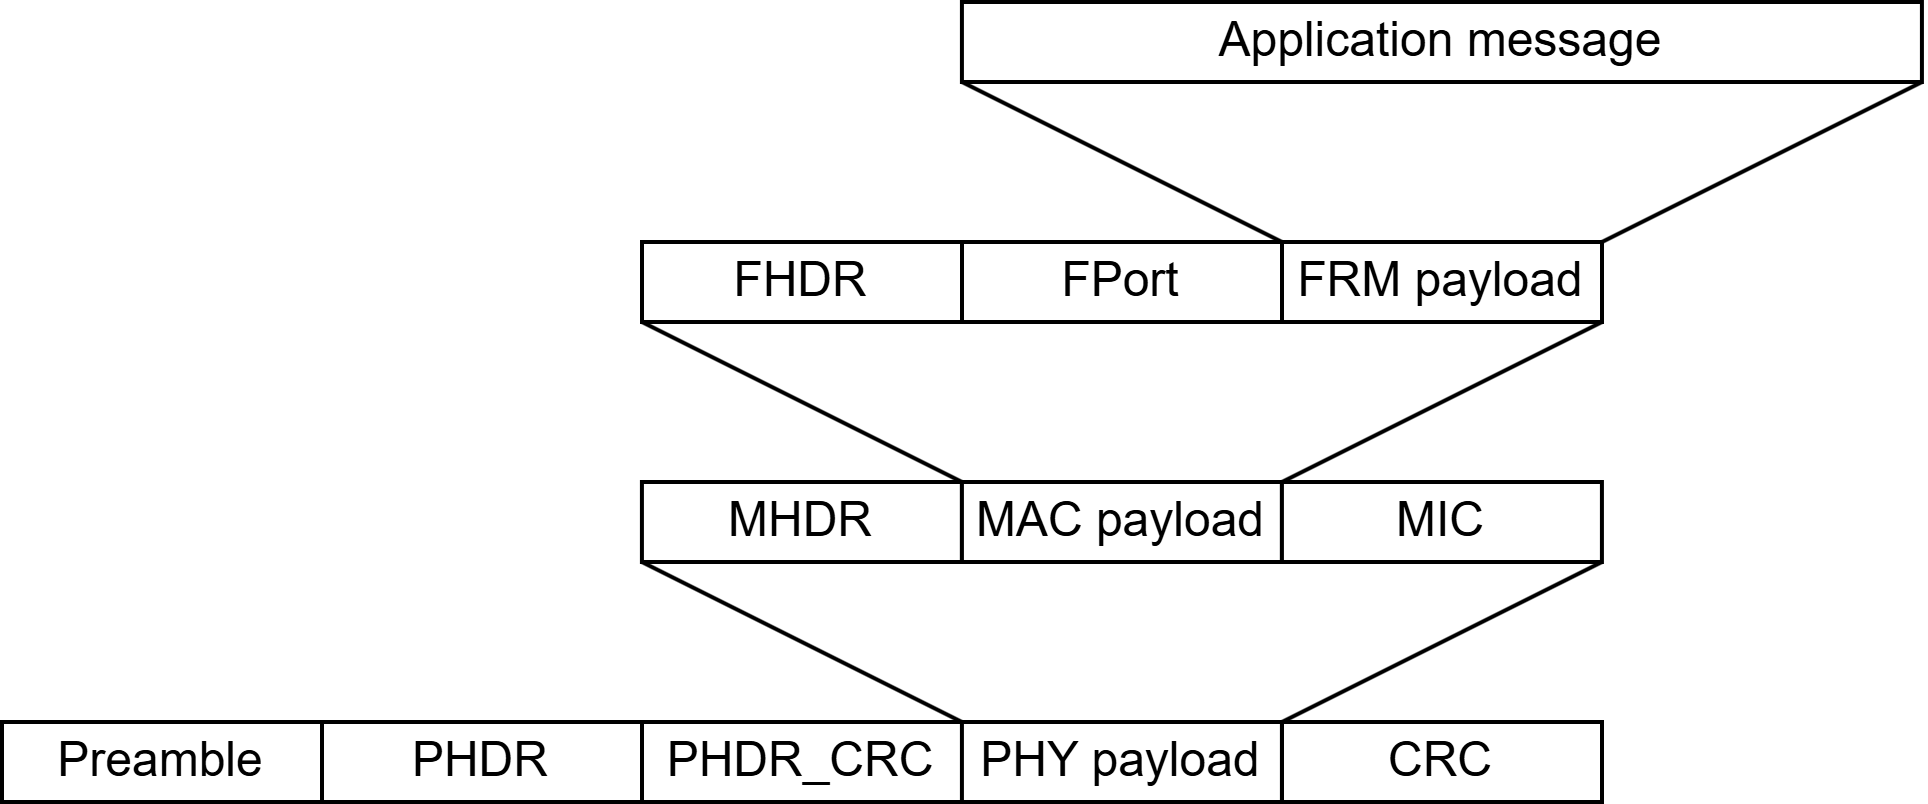
\includegraphics[width=0.5\linewidth]{images/iot12.png}
    \caption{LoraWAN messages}
\end{figure}

\subsection{Uplink}
Uplink transmissions in LoRaWAN follow an un-slotted ALOHA approach. 
When a confirmed message is transmitted but no acknowledgment (ACK) is received, the message is retransmitted after a randomly chosen delay.

LoraWAN does not rely on explicit channel feedback. 
Instead, devices infer success or failure based on ACK receipt. 
Time is modeled as continuous, and packets are transmitted as soon as they are queued. 
Retransmissions are delayed by a randomized backoff interval.

To model network performance, it is assumed that:
\begin{itemize}
    \item Traffic is stationary, meaning input and output rates are equal. 
    \item Packet arrivals follow a Poisson distribution with rate $\lambda$. 
    \item Each packet transmission lasts $T$ seconds.
    \item The total channel load is $G=\lambda T$.
\end{itemize}
\noindent The success probability $\Pr_s$, i.e., the probability that no other transmission overlaps within a vulnerable period $2T$, is:
\[\Pr_s=\Pr(N(t-T,t+T)=0)=e^{-2G}\]
\noindent The throughput $S$, defined as successful transmissions per time unit, becomes:
\[S=\text{G}\Pr_s=Ge^{-2G}\]
\noindent This relationship illustrates the classic ALOHA performance curve, with a peak throughput at $G=0.5$, beyond which performance degrades due to increasing collisions. 